% Graphic for TeX using PGF
% Title: /home/jnicolaschc/GitHub/Teoría de Telecominicaciones I /ttl1_trabajo3/Documentos/desarrollo/codigofuente/pgf/traslape1.dia
% Creator: Dia v0.97+git
% CreationDate: Fri Aug 20 23:46:44 2021
% For: jnicolaschc
% \usepackage{tikz}
% The following commands are not supported in PSTricks at present
% We define them conditionally, so when they are implemented,
% this pgf file will use them.
\begin{figure}[]
	\centering
	\ifx\du\undefined
		\newlength{\du}
	\fi
	\setlength{\du}{15\unitlength}
	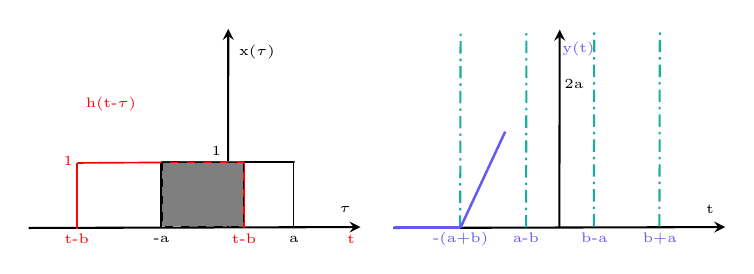
\begin{tikzpicture}[scale = 0.8]
		\pgftransformxscale{1.000000}
		\pgftransformyscale{-1.000000}
		\definecolor{dialinecolor}{rgb}{0.000000, 0.000000, 0.000000}
		\pgfsetstrokecolor{dialinecolor}
		\pgfsetstrokeopacity{1.000000}
		\definecolor{diafillcolor}{rgb}{1.000000, 1.000000, 1.000000}
		\pgfsetfillcolor{diafillcolor}
		\pgfsetfillopacity{1.000000}
		\pgfsetlinewidth{0.050000\du}
		\pgfsetdash{}{0pt}
		\pgfsetbuttcap
		{
			\definecolor{diafillcolor}{rgb}{0.000000, 0.000000, 0.000000}
			\pgfsetfillcolor{diafillcolor}
			\pgfsetfillopacity{1.000000}
			% was here!!!
			\pgfsetarrowsend{stealth}
			\definecolor{dialinecolor}{rgb}{0.000000, 0.000000, 0.000000}
			\pgfsetstrokecolor{dialinecolor}
			\pgfsetstrokeopacity{1.000000}
			\draw (40.002568\du,15.011800\du)--(40.014068\du,9.028390\du);
		}
		\pgfsetlinewidth{0.050000\du}
		\pgfsetdash{}{0pt}
		\pgfsetbuttcap
		{
			\definecolor{diafillcolor}{rgb}{0.000000, 0.000000, 0.000000}
			\pgfsetfillcolor{diafillcolor}
			\pgfsetfillopacity{1.000000}
			% was here!!!
			\pgfsetarrowsend{stealth}
			\definecolor{dialinecolor}{rgb}{0.000000, 0.000000, 0.000000}
			\pgfsetstrokecolor{dialinecolor}
			\pgfsetstrokeopacity{1.000000}
			\draw (34.004392\du,15.022957\du)--(43.996117\du,14.995695\du);
		}
		\pgfsetlinewidth{0.040000\du}
		\pgfsetdash{}{0pt}
		\pgfsetbuttcap
		{
			\definecolor{diafillcolor}{rgb}{0.000000, 0.000000, 0.000000}
			\pgfsetfillcolor{diafillcolor}
			\pgfsetfillopacity{1.000000}
			% was here!!!
			\definecolor{dialinecolor}{rgb}{0.000000, 0.000000, 0.000000}
			\pgfsetstrokecolor{dialinecolor}
			\pgfsetstrokeopacity{1.000000}
			\draw (37.996668\du,15.011800\du)--(37.996668\du,13.028800\du);
		}
		\pgfsetlinewidth{0.040000\du}
		\pgfsetdash{}{0pt}
		\pgfsetbuttcap
		{
			\definecolor{diafillcolor}{rgb}{0.000000, 0.000000, 0.000000}
			\pgfsetfillcolor{diafillcolor}
			\pgfsetfillopacity{1.000000}
			% was here!!!
			\definecolor{dialinecolor}{rgb}{0.000000, 0.000000, 0.000000}
			\pgfsetstrokecolor{dialinecolor}
			\pgfsetstrokeopacity{1.000000}
			\draw (41.980368\du,14.986000\du)--(41.980368\du,13.002900\du);
		}
		\pgfsetlinewidth{0.040000\du}
		\pgfsetdash{}{0pt}
		\pgfsetbuttcap
		{
			\definecolor{diafillcolor}{rgb}{0.000000, 0.000000, 0.000000}
			\pgfsetfillcolor{diafillcolor}
			\pgfsetfillopacity{1.000000}
			% was here!!!
			\definecolor{dialinecolor}{rgb}{0.000000, 0.000000, 0.000000}
			\pgfsetstrokecolor{dialinecolor}
			\pgfsetstrokeopacity{1.000000}
			\draw (37.996668\du,13.034500\du)--(42.011054\du,13.038374\du);
		}
		% setfont left to latex
		\definecolor{dialinecolor}{rgb}{0.000000, 0.000000, 0.000000}
		\pgfsetstrokecolor{dialinecolor}
		\pgfsetstrokeopacity{1.000000}
		\definecolor{diafillcolor}{rgb}{0.000000, 0.000000, 0.000000}
		\pgfsetfillcolor{diafillcolor}
		\pgfsetfillopacity{1.000000}
		\node[anchor=base,inner sep=0pt, outer sep=0pt,color=dialinecolor] at (38.000033\du,15.471175\du){\tiny -a};
		% setfont left to latex
		\definecolor{dialinecolor}{rgb}{0.000000, 0.000000, 0.000000}
		\pgfsetstrokecolor{dialinecolor}
		\pgfsetstrokeopacity{1.000000}
		\definecolor{diafillcolor}{rgb}{0.000000, 0.000000, 0.000000}
		\pgfsetfillcolor{diafillcolor}
		\pgfsetfillopacity{1.000000}
		\node[anchor=base,inner sep=0pt, outer sep=0pt,color=dialinecolor] at (41.991133\du,15.458075\du){\tiny a};
		% setfont left to latex
		\definecolor{dialinecolor}{rgb}{0.000000, 0.000000, 0.000000}
		\pgfsetstrokecolor{dialinecolor}
		\pgfsetstrokeopacity{1.000000}
		\definecolor{diafillcolor}{rgb}{0.000000, 0.000000, 0.000000}
		\pgfsetfillcolor{diafillcolor}
		\pgfsetfillopacity{1.000000}
		\node[anchor=base east,inner sep=0pt, outer sep=0pt,color=dialinecolor] at (39.799158\du,12.850010\du){\tiny 1};
		% setfont left to latex
		\definecolor{dialinecolor}{rgb}{0.000000, 0.000000, 0.000000}
		\pgfsetstrokecolor{dialinecolor}
		\pgfsetstrokeopacity{1.000000}
		\definecolor{diafillcolor}{rgb}{0.000000, 0.000000, 0.000000}
		\pgfsetfillcolor{diafillcolor}
		\pgfsetfillopacity{1.000000}
		\node[anchor=base,inner sep=0pt, outer sep=0pt,color=dialinecolor] at (43.532653\du,14.548198\du){\tiny $\tau$};
		% setfont left to latex
		\definecolor{dialinecolor}{rgb}{0.000000, 0.000000, 0.000000}
		\pgfsetstrokecolor{dialinecolor}
		\pgfsetstrokeopacity{1.000000}
		\definecolor{diafillcolor}{rgb}{0.000000, 0.000000, 0.000000}
		\pgfsetfillcolor{diafillcolor}
		\pgfsetfillopacity{1.000000}
		\node[anchor=base west,inner sep=0pt,outer sep=0pt,color=dialinecolor] at (40.337268\du,9.823361\du){\tiny x($\tau$)};
		\pgfsetlinewidth{0.040000\du}
		\pgfsetdash{}{0pt}
		\pgfsetbuttcap
		{
			\definecolor{diafillcolor}{rgb}{1.000000, 0.000000, 0.000000}
			\pgfsetfillcolor{diafillcolor}
			\pgfsetfillopacity{1.000000}
			% was here!!!
			\definecolor{dialinecolor}{rgb}{1.000000, 0.000000, 0.000000}
			\pgfsetstrokecolor{dialinecolor}
			\pgfsetstrokeopacity{1.000000}
			\draw (35.467140\du,15.042600\du)--(35.467140\du,13.059600\du);
		}
		\pgfsetlinewidth{0.040000\du}
		\pgfsetdash{}{0pt}
		\pgfsetbuttcap
		{
			\definecolor{diafillcolor}{rgb}{1.000000, 0.000000, 0.000000}
			\pgfsetfillcolor{diafillcolor}
			\pgfsetfillopacity{1.000000}
			% was here!!!
			\definecolor{dialinecolor}{rgb}{1.000000, 0.000000, 0.000000}
			\pgfsetstrokecolor{dialinecolor}
			\pgfsetstrokeopacity{1.000000}
			\draw (40.482540\du,15.016700\du)--(40.482540\du,13.033700\du);
		}
		\pgfsetlinewidth{0.040000\du}
		\pgfsetdash{}{0pt}
		\pgfsetbuttcap
		{
			\definecolor{diafillcolor}{rgb}{1.000000, 0.000000, 0.000000}
			\pgfsetfillcolor{diafillcolor}
			\pgfsetfillopacity{1.000000}
			% was here!!!
			\definecolor{dialinecolor}{rgb}{1.000000, 0.000000, 0.000000}
			\pgfsetstrokecolor{dialinecolor}
			\pgfsetstrokeopacity{1.000000}
			\draw (35.467140\du,13.065300\du)--(40.476440\du,13.034500\du);
		}
		% setfont left to latex
		\definecolor{dialinecolor}{rgb}{1.000000, 0.000000, 0.000000}
		\pgfsetstrokecolor{dialinecolor}
		\pgfsetstrokeopacity{1.000000}
		\definecolor{diafillcolor}{rgb}{1.000000, 0.000000, 0.000000}
		\pgfsetfillcolor{diafillcolor}
		\pgfsetfillopacity{1.000000}
		\node[anchor=base,inner sep=0pt, outer sep=0pt,color=dialinecolor] at (35.455740\du,15.502231\du){\tiny t-b};
		% setfont left to latex
		\definecolor{dialinecolor}{rgb}{1.000000, 0.000000, 0.000000}
		\pgfsetstrokecolor{dialinecolor}
		\pgfsetstrokeopacity{1.000000}
		\definecolor{diafillcolor}{rgb}{1.000000, 0.000000, 0.000000}
		\pgfsetfillcolor{diafillcolor}
		\pgfsetfillopacity{1.000000}
		\node[anchor=base,inner sep=0pt, outer sep=0pt,color=dialinecolor] at (40.489840\du,15.502231\du){\tiny t-b};
		% setfont left to latex
		\definecolor{dialinecolor}{rgb}{1.000000, 0.000000, 0.000000}
		\pgfsetstrokecolor{dialinecolor}
		\pgfsetstrokeopacity{1.000000}
		\definecolor{diafillcolor}{rgb}{1.000000, 0.000000, 0.000000}
		\pgfsetfillcolor{diafillcolor}
		\pgfsetfillopacity{1.000000}
		\node[anchor=base east,inner sep=0pt, outer sep=0pt,color=dialinecolor] at (35.332740\du,13.134346\du){\tiny 1};
		% setfont left to latex
		\definecolor{dialinecolor}{rgb}{1.000000, 0.000000, 0.000000}
		\pgfsetstrokecolor{dialinecolor}
		\pgfsetstrokeopacity{1.000000}
		\definecolor{diafillcolor}{rgb}{1.000000, 0.000000, 0.000000}
		\pgfsetfillcolor{diafillcolor}
		\pgfsetfillopacity{1.000000}
		\node[anchor=base west,inner sep=0pt,outer sep=0pt,color=dialinecolor] at (35.723728\du,11.406141\du){\tiny h(t-$\tau$)};
		% setfont left to latex
		\definecolor{dialinecolor}{rgb}{1.000000, 0.000000, 0.000000}
		\pgfsetstrokecolor{dialinecolor}
		\pgfsetstrokeopacity{1.000000}
		\definecolor{diafillcolor}{rgb}{1.000000, 0.000000, 0.000000}
		\pgfsetfillcolor{diafillcolor}
		\pgfsetfillopacity{1.000000}
		\node[anchor=base,inner sep=0pt, outer sep=0pt,color=dialinecolor] at (43.715072\du,15.482150\du){\tiny t};
		\pgfsetlinewidth{0.030000\du}
		\pgfsetdash{{0.200000\du}{0.200000\du}}{0\du}
		\pgfsetmiterjoin
		\pgfsetbuttcap
		{\pgfsetcornersarced{\pgfpoint{0.000000\du}{0.000000\du}}\definecolor{diafillcolor}{rgb}{0.498039, 0.498039, 0.498039}
			\pgfsetfillcolor{diafillcolor}
			\pgfsetfillopacity{1.000000}
			\fill (38.017810\du,13.053239\du)--(38.017810\du,14.977525\du)--(40.465090\du,14.977525\du)--(40.465090\du,13.053239\du)--cycle;
		}{\pgfsetcornersarced{\pgfpoint{0.000000\du}{0.000000\du}}\definecolor{dialinecolor}{rgb}{0.000000, 0.000000, 0.000000}
			\pgfsetstrokecolor{dialinecolor}
			\pgfsetstrokeopacity{1.000000}
			\draw (38.017810\du,13.053239\du)--(38.017810\du,14.977525\du)--(40.465090\du,14.977525\du)--(40.465090\du,13.053239\du)--cycle;
		}\pgfsetlinewidth{0.050000\du}
		\pgfsetdash{}{0pt}
		\pgfsetbuttcap
		{
			\definecolor{diafillcolor}{rgb}{0.000000, 0.000000, 0.000000}
			\pgfsetfillcolor{diafillcolor}
			\pgfsetfillopacity{1.000000}
			% was here!!!
			\pgfsetarrowsend{stealth}
			\definecolor{dialinecolor}{rgb}{0.000000, 0.000000, 0.000000}
			\pgfsetstrokecolor{dialinecolor}
			\pgfsetstrokeopacity{1.000000}
			\draw (44.986279\du,15.023266\du)--(54.978004\du,14.996003\du);
		}
		\pgfsetlinewidth{0.050000\du}
		\pgfsetdash{}{0pt}
		\pgfsetbuttcap
		{
			\definecolor{diafillcolor}{rgb}{0.000000, 0.000000, 0.000000}
			\pgfsetfillcolor{diafillcolor}
			\pgfsetfillopacity{1.000000}
			% was here!!!
			\pgfsetarrowsend{stealth}
			\definecolor{dialinecolor}{rgb}{0.000000, 0.000000, 0.000000}
			\pgfsetstrokecolor{dialinecolor}
			\pgfsetstrokeopacity{1.000000}
			\draw (49.982142\du,15.009634\du)--(49.993878\du,9.052459\du);
		}
		\pgfsetlinewidth{0.050000\du}
		\pgfsetdash{{0.300000\du}{0.120000\du}{0.060000\du}{0.120000\du}}{0cm}
		\pgfsetbuttcap
		{
			\definecolor{diafillcolor}{rgb}{0.101961, 0.682353, 0.623529}
			\pgfsetfillcolor{diafillcolor}
			\pgfsetfillopacity{1.000000}
			% was here!!!
			\definecolor{dialinecolor}{rgb}{0.101961, 0.682353, 0.623529}
			\pgfsetstrokecolor{dialinecolor}
			\pgfsetstrokeopacity{1.000000}
			\draw (46.996410\du,15.021052\du)--(47.008146\du,9.063877\du);
		}
		\pgfsetlinewidth{0.050000\du}
		\pgfsetdash{{0.300000\du}{0.120000\du}{0.060000\du}{0.120000\du}}{0cm}
		\pgfsetbuttcap
		{
			\definecolor{diafillcolor}{rgb}{0.101961, 0.682353, 0.623529}
			\pgfsetfillcolor{diafillcolor}
			\pgfsetfillopacity{1.000000}
			% was here!!!
			\definecolor{dialinecolor}{rgb}{0.101961, 0.682353, 0.623529}
			\pgfsetstrokecolor{dialinecolor}
			\pgfsetstrokeopacity{1.000000}
			\draw (48.980224\du,15.007421\du)--(48.991960\du,9.050246\du);
		}
		\pgfsetlinewidth{0.050000\du}
		\pgfsetdash{{0.300000\du}{0.120000\du}{0.060000\du}{0.120000\du}}{0cm}
		\pgfsetbuttcap
		{
			\definecolor{diafillcolor}{rgb}{0.101961, 0.682353, 0.623529}
			\pgfsetfillcolor{diafillcolor}
			\pgfsetfillopacity{1.000000}
			% was here!!!
			\definecolor{dialinecolor}{rgb}{0.101961, 0.682353, 0.623529}
			\pgfsetstrokecolor{dialinecolor}
			\pgfsetstrokeopacity{1.000000}
			\draw (51.022189\du,14.980158\du)--(51.033925\du,9.022983\du);
		}
		\pgfsetlinewidth{0.050000\du}
		\pgfsetdash{{0.300000\du}{0.120000\du}{0.060000\du}{0.120000\du}}{0cm}
		\pgfsetbuttcap
		{
			\definecolor{diafillcolor}{rgb}{0.101961, 0.682353, 0.623529}
			\pgfsetfillcolor{diafillcolor}
			\pgfsetfillopacity{1.000000}
			% was here!!!
			\definecolor{dialinecolor}{rgb}{0.101961, 0.682353, 0.623529}
			\pgfsetstrokecolor{dialinecolor}
			\pgfsetstrokeopacity{1.000000}
			\draw (52.995998\du,14.980158\du)--(53.007734\du,9.022983\du);
		}
		\pgfsetlinewidth{0.060000\du}
		\pgfsetdash{}{0pt}
		\pgfsetbuttcap
		{
			\definecolor{diafillcolor}{rgb}{0.396078, 0.345098, 0.960784}
			\pgfsetfillcolor{diafillcolor}
			\pgfsetfillopacity{1.000000}
			% was here!!!
			\definecolor{dialinecolor}{rgb}{0.396078, 0.345098, 0.960784}
			\pgfsetstrokecolor{dialinecolor}
			\pgfsetstrokeopacity{1.000000}
			\draw (45.005231\du,15.011197\du)--(46.988241\du,15.011197\du);
		}
		\pgfsetlinewidth{0.060000\du}
		\pgfsetdash{}{0pt}
		\pgfsetbuttcap
		{
			\definecolor{diafillcolor}{rgb}{0.396078, 0.345098, 0.960784}
			\pgfsetfillcolor{diafillcolor}
			\pgfsetfillopacity{1.000000}
			% was here!!!
			\definecolor{dialinecolor}{rgb}{0.396078, 0.345098, 0.960784}
			\pgfsetstrokecolor{dialinecolor}
			\pgfsetstrokeopacity{1.000000}
			\draw (47.011166\du,14.999735\du)--(48.352276\du,12.122651\du);
		}
		% setfont left to latex
		\definecolor{dialinecolor}{rgb}{0.396078, 0.345098, 0.960784}
		\pgfsetstrokecolor{dialinecolor}
		\pgfsetstrokeopacity{1.000000}
		\definecolor{diafillcolor}{rgb}{0.396078, 0.345098, 0.960784}
		\pgfsetfillcolor{diafillcolor}
		\pgfsetfillopacity{1.000000}
		\node[anchor=base,inner sep=0pt, outer sep=0pt,color=dialinecolor] at (47.009480\du,15.461516\du){\tiny -(a+b)};
		% setfont left to latex
		\definecolor{dialinecolor}{rgb}{0.396078, 0.345098, 0.960784}
		\pgfsetstrokecolor{dialinecolor}
		\pgfsetstrokeopacity{1.000000}
		\definecolor{diafillcolor}{rgb}{0.396078, 0.345098, 0.960784}
		\pgfsetfillcolor{diafillcolor}
		\pgfsetfillopacity{1.000000}
		\node[anchor=base,inner sep=0pt, outer sep=0pt,color=dialinecolor] at (48.976569\du,15.450054\du){\tiny a-b};
		% setfont left to latex
		\definecolor{dialinecolor}{rgb}{0.396078, 0.345098, 0.960784}
		\pgfsetstrokecolor{dialinecolor}
		\pgfsetstrokeopacity{1.000000}
		\definecolor{diafillcolor}{rgb}{0.396078, 0.345098, 0.960784}
		\pgfsetfillcolor{diafillcolor}
		\pgfsetfillopacity{1.000000}
		\node[anchor=base,inner sep=0pt, outer sep=0pt,color=dialinecolor] at (51.037524\du,15.451660\du){\tiny b-a};
		% setfont left to latex
		\definecolor{dialinecolor}{rgb}{0.396078, 0.345098, 0.960784}
		\pgfsetstrokecolor{dialinecolor}
		\pgfsetstrokeopacity{1.000000}
		\definecolor{diafillcolor}{rgb}{0.396078, 0.345098, 0.960784}
		\pgfsetfillcolor{diafillcolor}
		\pgfsetfillopacity{1.000000}
		\node[anchor=base,inner sep=0pt, outer sep=0pt,color=dialinecolor] at (53.006778\du,15.451660\du){\tiny b+a};
		% setfont left to latex
		\definecolor{dialinecolor}{rgb}{0.000000, 0.000000, 0.000000}
		\pgfsetstrokecolor{dialinecolor}
		\pgfsetstrokeopacity{1.000000}
		\definecolor{diafillcolor}{rgb}{0.000000, 0.000000, 0.000000}
		\pgfsetfillcolor{diafillcolor}
		\pgfsetfillopacity{1.000000}
		\node[anchor=base,inner sep=0pt, outer sep=0pt,color=dialinecolor] at (54.525875\du,14.580511\du){\tiny t};
		% setfont left to latex
		\definecolor{dialinecolor}{rgb}{0.000000, 0.000000, 0.000000}
		\pgfsetstrokecolor{dialinecolor}
		\pgfsetstrokeopacity{1.000000}
		\definecolor{diafillcolor}{rgb}{0.000000, 0.000000, 0.000000}
		\pgfsetfillcolor{diafillcolor}
		\pgfsetfillopacity{1.000000}
		\node[anchor=base,inner sep=0pt, outer sep=0pt,color=dialinecolor] at (50.420842\du,10.820816\du){\tiny 2a};
		% setfont left to latex
		\definecolor{dialinecolor}{rgb}{0.396078, 0.345098, 0.960784}
		\pgfsetstrokecolor{dialinecolor}
		\pgfsetstrokeopacity{1.000000}
		\definecolor{diafillcolor}{rgb}{0.396078, 0.345098, 0.960784}
		\pgfsetfillcolor{diafillcolor}
		\pgfsetfillopacity{1.000000}
		\node[anchor=base,inner sep=0pt, outer sep=0pt,color=dialinecolor] at (50.558392\du,9.743342\du){\tiny y(t)};
	\end{tikzpicture}
	\caption{}
	\label{}
\end{figure}
